\documentclass[a4paper,12pt, titlepage]{article} 
\usepackage{geometry}           % пакет для задания полей страницы командой \geometry
\geometry{left=3cm,right=1.5cm,top=2cm,bottom=2cm}
\usepackage[utf8]{inputenc}
\usepackage[english,russian]{babel}
\usepackage{amsmath}
%\usepackage{amsthm}
%\usepackage{cmap}
\usepackage{indentfirst}
\usepackage{a4wide,amssymb}
%\usepackage[pdftex]{graphicx}
%\usepackage[pdftex]{graphics}
%\usepackage{wrapfig}
%\linespread{1.3}                % полтора интервала. Если 1.6, то два интервала
\pagestyle{plain}               % номерует страницы

\usepackage{graphicx}
\renewcommand{\topfraction}{1}
\renewcommand{\textfraction}{0}


%opening
\title{Коррекция многогранников \\ по теневым контурам в целом \\ (план работы)}
\author{Палачев Илья}



\begin{document}


\maketitle

\tableofcontents

\section{Постановка задачи}

\begin{flushleft}
В данной работе рассматривается проблема уточнения многогранника, построенного по 
набору теневых контуров.

Пусть имеется набор $S_{1}, S_{2}, S_{3}, \ldots, S_{N}$ теневых контуров,
полученных в результате фотографирования реального камня, а также алгоритм,
позволяющий построить трехмерную модель камня (многогранник) с некоторой 
точностью. 

Тогда можно вновь построить теневые контуры для построенного многоранника
и сравнить их с исходными данными. Разница между исходными и построенными контурами
определяет точность построения модели.

Требуется подвинуть вершины и грани этого многогранника таким образом, чтобы 
улучшить (по возможности оптимально) приближение модели, т. е. улучшить наложение 
построенных контуров на исходные.
\end{flushleft}

\begin{flushleft}
 Теневые контуры $S_{k}$ рассматриваются как упорядоченные последовательности ребер
$\tilde{e}_{k1}, \tilde{e}_{k2}, \ldots, \tilde{e}_{kn_{k}}$, 
лежащих в заданной плоскости (плоскости проекции $\tilde{\pi}_{k}$). 
Каждому такому ребру соответствует некоторое ребро $e_{s(ki)}$ на многограннике.

Будем минимизировать следующий функционал:

\begin{equation}
\sum\limits_{k = 1}^{N}\sum\limits_{i = 1}^{n_{k}} \rho (\tilde{e}_{ki} , pr_{k}(e_{s(ki)})) 
\to min
\end{equation}

где $pr_{k} : \mathbb{R}^{3} \to \tilde{\pi}_{k}$ -- проектор на плоскость 
$\tilde{\pi}_{k}$, $\rho$ -- некоторая метрика расстояния между отрезками на плоскости.
\end{flushleft}





\section{Методы решения}

\begin{flushleft}
 Пусть ребро $e_{s(ki)}$, соединяющее грани $\pi_{1}$ и $\pi_{2}$ 
 есть прообраз ребра $\tilde{e}_{ki}$ 
 в плоскости $\tilde{\pi}_{k}$ при отображении $pr_{k}$.  Данное отображение есть проектор
 вдоль оси проектирования $\nu_{k}$ -- нормали к плоскости $\tilde{\pi}_{k}$. 
 
 Построим плоскость $\alpha_{ki}$, проходящую через ребро  
 $e_{s(ki)}$ и параллельную оси $\nu_{k}$.
 Тогда в качестве расстояния между ребрами можно взять сумму расстояний от вершин ребра
 $\tilde{e}_{ki}$ до плоскости $\alpha_{ki}$:


 \begin{multline}
  \rho(e_{s(ki)}, \tilde{e}_{ki}) = \rho (\tilde{A}_{ki1}, \alpha_{ki}) + 
  \rho (\tilde{A}_{ki2}, \alpha_{ki}) = 
  \frac{|a_{ki} x_{ki1} + b_{ki} y_{ki1} + c_{ki} z_{ki1} + d_{ki}|}
  {\sqrt{a_{ki}^{2} + b_{ki}^{2} + c_{ki}^{2}}} + \\ +
  \frac{|a_{ki} x_{ki2} + b_{ki} y_{ki2} + c_{ki} z_{ki2} + d_{ki}|}
  {\sqrt{a_{ki}^{2} + b_{ki}^{2} + c_{ki}^{2}}},
 \end{multline}
 
 где $\tilde{A}_{ki1}$ и $\tilde{A}_{ki2}$ -- вершины ребра $\tilde{e}_{ki}$
\end{flushleft}

\begin{flushleft}
  \begin{figure}[ht]
    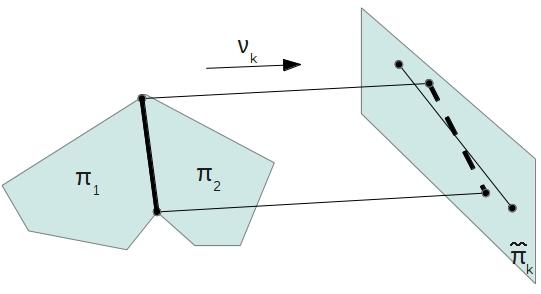
\includegraphics[clip, width=10cm]{pi1pi2.jpg}
    \caption{Соответствие между ребрами}\label{pi1pi2}
  \end{figure}
\end{flushleft}

\begin{flushleft}
 Коэффициенты плоскости $\alpha_{ki}$ должно выразить в терминах переменных, относительно
 которых минимизируется функционал, то есть через коэффициенты этих плоскостей многогранника. 
 Ребро $e_{s(ki)}$ лежит в плоскостях $\pi_{1}$, $\pi_{2}$ и $\alpha_{ki}$, поэтому оно
 перпендикулярно нормалям этих плоскотей: $n_{1}$, $n_{2}$ и $n_{ki}$. Следовательно, эти 
 три нормали лежат в одной плоскости. Нормали $n_{1}$, $n_{2}$ не совпадают, значит, они 
 образуют базис в плоскости, перепендикулярной ребру $e_{s(ki)}$, и вектор $n_{ki}$ можно
 представить в виде их линейной комбинации. Для удобства положим:
\end{flushleft}

\begin{flushleft}
 $$ n_{ki} = \gamma n_{1} + (1 - \gamma) n_{2} $$
 $$\begin{pmatrix} a \\ b \\ c \end{pmatrix} = 
 \gamma \begin{pmatrix} a_{1} \\ b_{1} \\ c_{1} \end{pmatrix} + 
 (1 - \gamma) \begin{pmatrix} a_{2} \\ b_{2} \\ c_{2} \end{pmatrix} 
 $$
\end{flushleft}

\begin{flushleft}
 Отсюда можно выразить коэффициент $\gamma$:
 
\begin{equation}
 \gamma = - \frac{a_{2}\nu_{x} + b_{2}\nu_{y} + c_{2}\nu_{z}}
 {(a_{1} - a_{2})\nu_{x} + (b_{1} - b_{2})\nu_{y} + (c_{1} - c_{2})\nu_{z}}
\end{equation}
\end{flushleft}

\begin{flushleft}
 Заметим, что в этом случае выражается и коэффициент $d$, так как иначе три плоскости 
 не могут иметь общую прямую.
 $d = \gamma d_{1} + (1 - \gamma) d_{2}$
\end{flushleft}

\begin{flushleft}
 Теперь осталось только подставить эти коэффициенты в выражение для функционала.
 
 \begin{multline}
    I = \sum\limits_{i = 1}^{K} \sum\limits_{\{j:e_{i} \rightsquigarrow pr_{j}\}}
  \{
    [ 
      (\gamma_{ij} a_{s(ij1)} + (1 - \gamma_{ij}) a_{s(ij2)}) \tilde{x}_{l(ij1)} + 
      (\gamma_{ij} b_{s(ij1)} + (1 - \gamma_{ij}) b_{s(ij2)}) \tilde{y}_{l(ij1)} + \\ +
      (\gamma_{ij} c_{s(ij1)} + (1 - \gamma_{ij}) c_{s(ij2)}) \tilde{z}_{l(ij1)} + 
      (\gamma_{ij} d_{s(ij1)} + (1 - \gamma_{ij}) d_{s(ij2)}) 
    ]^{2} + \\
    [ 
      (\gamma_{ij} a_{s(ij1)} + (1 - \gamma_{ij}) a_{s(ij2)}) \tilde{x}_{l(ij2)} + 
      (\gamma_{ij} b_{s(ij1)} + (1 - \gamma_{ij}) b_{s(ij2)}) \tilde{y}_{l(ij2)} + \\ +
      (\gamma_{ij} c_{s(ij1)} + (1 - \gamma_{ij}) c_{s(ij2)}) \tilde{z}_{l(ij2)} + 
      (\gamma_{ij} d_{s(ij1)} + (1 - \gamma_{ij}) d_{s(ij2)}) 
    ]^{2}\}
 \end{multline}
 В этом выражении индекс $i$ пробегает по номерам всех ребер, а индекс $j$ -- по номерам всех 
 теневых контуров, в котором видно текущее $i$-е ребро $e_{i}$. $s(ij1)$ и $s(ij2)$ обозначают номера
 плоскостей многогранника, граничащих по ребру $e_{i}$, а $l(ij1)$ и $l(ij2)$ -- номера вершин
 $j$-го теневого контура, в которые проецируется $e_{i}$.
\end{flushleft}

\begin{flushleft}
 Частная производная этого функционала будет иметь следующий вид:
\end{flushleft}

$$
\begin{aligned}
  \frac{\partial I}{\partial a_{k}} = 
  \sum\limits_{\{i : e_{i} \in \pi_{k}\}} \sum\limits_{\{j:e_{i} \rightsquigarrow pr_{j}\}}
  \{
    2 \gamma_{ij} 
    [
      (\gamma_{ij} a_{k} + (1 - \gamma_{ij}) a_{s(ij2)}) 
      (\tilde{x}_{l(ij1)}^{2} + \tilde{x}_{l(ij2)}^{2}) + \\ +
      (\gamma_{ij} b_{k} + (1 - \gamma_{ij}) b_{s(ij2)}) 
      (\tilde{x}_{l(ij1)} \tilde{y}_{l(ij1)} + \tilde{x}_{l(ij2)} \tilde{y}_{l(ij2)}) + \\ +
      (\gamma_{ij} c_{k} + (1 - \gamma_{ij}) c_{s(ij2)}) 
      (\tilde{x}_{l(ij1)} \tilde{z}_{l(ij1)} + \tilde{x}_{l(ij2)} \tilde{z}_{l(ij2)}) + \\ + 
      (\gamma_{ij} d_{k} + (1 - \gamma_{ij}) d_{s(ij2)}) 
      (\tilde{x}_{l(ij1)} + \tilde{x}_{l(ij2)})
    ]
  \}
\end{aligned}
$$

\begin{flushleft}
 Если рассматривать также случай бликовых контуров, то функционал примет несколько более сложный вид:
\end{flushleft}

 \begin{multline}
  I = \sum\limits_{i = 1}^{K} \sum\limits_{\{j:e_{i} \rightsquigarrow pr_{j}\}}
  \{
    [ 
      (\gamma_{ij} a_{s(ij1)} + (1 - \gamma_{ij}) a_{s(ij2)}) \tilde{x}_{l(ij1)} + 
      (\gamma_{ij} b_{s(ij1)} + (1 - \gamma_{ij}) b_{s(ij2)}) \tilde{y}_{l(ij1)} + \\ +
      (\gamma_{ij} c_{s(ij1)} + (1 - \gamma_{ij}) c_{s(ij2)}) \tilde{z}_{l(ij1)} + 
      (\gamma_{ij} d_{s(ij1)} + (1 - \gamma_{ij}) d_{s(ij2)}) 
    ]^{2} + \\
    [ 
      (\gamma_{ij} a_{s(ij1)} + (1 - \gamma_{ij}) a_{s(ij2)}) \tilde{x}_{l(ij2)} + 
      (\gamma_{ij} b_{s(ij1)} + (1 - \gamma_{ij}) b_{s(ij2)}) \tilde{y}_{l(ij2)} + \\ +
      (\gamma_{ij} c_{s(ij1)} + (1 - \gamma_{ij}) c_{s(ij2)}) \tilde{z}_{l(ij2)} + 
      (\gamma_{ij} d_{s(ij1)} + (1 - \gamma_{ij}) d_{s(ij2)}) 
    ]^{2}\} + \\ +
    \sum\limits_{i = 1}^{K} \sum\limits_{\{j:e_{i} \rightsquigarrow pr^{b}_{j}\}}\{[ 
      (
	\gamma_{ij} 
	(-r_{zs^{b}(ij)} b_{s^{b}(ij1)} + r_{ys^{b}(ij)} c_{s^{b}(ij1)}) + 
	(1 - \gamma_{ij}) 
	(r_{zs^{b}(ij)} b_{s^{b}(ij2)} - r_{ys^{b}(ij)} c_{s^{b}(ij2)})
      ) \tilde{x}_{l^{b}(ij1)} + \\ +
      (
	\gamma_{ij} 
	(r_{zs^{b}(ij)} a_{s^{b}(ij1)} - r_{xs^{b}(ij)} c_{s^{b}(ij1)}) + 
	(1 - \gamma_{ij}) 
	(-r_{zs^{b}(ij)} a_{s^{b}(ij2)} + r_{xs^{b}(ij)} c_{s^{b}(ij2)})
      ) \tilde{y}_{l^{b}(ij1)} + \\ +
      (
	\gamma_{ij} 
	(-r_{ys^{b}(ij)} a_{s^{b}(ij1)} + r_{xs^{b}(ij)} b_{s^{b}(ij1)}) + 
	(1 - \gamma_{ij}) 
	(r_{ys^{b}(ij)} a_{s^{b}(ij2)} - r_{ys^{b}(ij)} b_{s^{b}(ij2)})
      ) \tilde{z}_{l^{b}(ij1)} + \\ +
      ((1 - \gamma_{ij}) - \gamma_{ij} (\vec{n}_{s^{b}(ij1)}, \vec{n}_{s^{b}(ij2)})) d_{s^{b}(ij1)} +
      (\gamma_{ij} - (1 - \gamma_{ij}) (\vec{n}_{s^{b}(ij1)}, \vec{n}_{s^{b}(ij2)})) d_{s^{b}(ij1)}
    ]^{2} + \\ +
    [ 
      (
	\gamma_{ij} 
	(-r_{zs^{b}(ij)} b_{s^{b}(ij1)} + r_{ys^{b}(ij)} c_{s^{b}(ij1)}) + 
	(1 - \gamma_{ij}) 
	(r_{zs^{b}(ij)} b_{s^{b}(ij2)} - r_{ys^{b}(ij)} c_{s^{b}(ij2)})
      ) \tilde{x}_{l^{b}(ij2)} + \\ +
      (
	\gamma_{ij} 
	(r_{zs^{b}(ij)} a_{s^{b}(ij1)} - r_{xs^{b}(ij)} c_{s^{b}(ij1)}) + 
	(1 - \gamma_{ij}) 
	(-r_{zs^{b}(ij)} a_{s^{b}(ij2)} + r_{xs^{b}(ij)} c_{s^{b}(ij2)})
      ) \tilde{y}_{l^{b}(ij2)} + \\ +
      (
	\gamma_{ij} 
	(-r_{ys^{b}(ij)} a_{s^{b}(ij1)} + r_{xs^{b}(ij)} b_{s^{b}(ij1)}) + 
	(1 - \gamma_{ij}) 
	(r_{ys^{b}(ij)} a_{s^{b}(ij2)} - r_{ys^{b}(ij)} b_{s^{b}(ij2)})
      ) \tilde{z}_{l^{b}(ij2)} + \\ +
      ((1 - \gamma_{ij}) - \gamma_{ij} (\vec{n}_{s^{b}(ij1)}, \vec{n}_{s^{b}(ij2)})) d_{s^{b}(ij1)} +
      (\gamma_{ij} - (1 - \gamma_{ij}) (\vec{n}_{s^{b}(ij1)}, \vec{n}_{s^{b}(ij2)})) d_{s^{b}(ij1)}  
    ]^{2}
  \} + \\ +
  \sum\limits_{k = 1}^{M}\lambda_{k}(a^{0}_{k} a_{k} + b^{0}_{k} b_{k} + c^{0}_{k} c_{k})
 \end{multline}





\section{Полученные результаты}


\end{document}
